
\section{IAD $\supseteq $ RDP $\times$ SMA }
%------------------------------------------------------------------------
\begin{frame}

\begin{center}
{\huge Capítulo 3 -- IAD $\supseteq $ RDP $\times$ SMA }
\end{center}

\end{frame}

%------------------------------------------------------------------------
\begin{frame} %[allowframebreaks=0.9]


\frametitle{O que vai ter neste capítulo}

\begin{itemize}
  \item Mais conceitos sobre SMA dentro da IAD ... vantagens etc
  \item Quando a RDP é mais interessante (e quando não é)
  \item Vantagens da SMA (e desvantagens com relação a RDP)
\end{itemize}


\end{frame}

%------------------------------------------------------------------------


\begin{frame} %[allowframebreaks=0.9]


\frametitle{Porque distribuir?}

\begin{itemize}
  \item Sistemas em geral são distribuídos \textbf{funcionalmente}
  \pause
  \begin{itemize}
    \item Devido uma especificação (a necessidade ou requisitos)
    \item Devido uma especialização
    \item Dividir e diminuir a complexidade $\rightarrow$ decompor o problema
    
  \end{itemize}

  \pause
  \item Sistemas em geral são distribuídos \textbf{fisicamente}
  \pause  
  \item Finalmente, na \textbf{resolução de problemas} (em geral): 
  há alguns cuja solução é inerentemente distribuída ou 
  fica mais fácil distribuindo!
  

\end{itemize}


\end{frame}
%------------------------------------------------------------------------

\begin{frame} %[allowframebreaks=0.9]

  \frametitle{Motivando o \textit{distribuído}}
        
\begin{figure}[!ht]
\centering
%\includegraphics{}
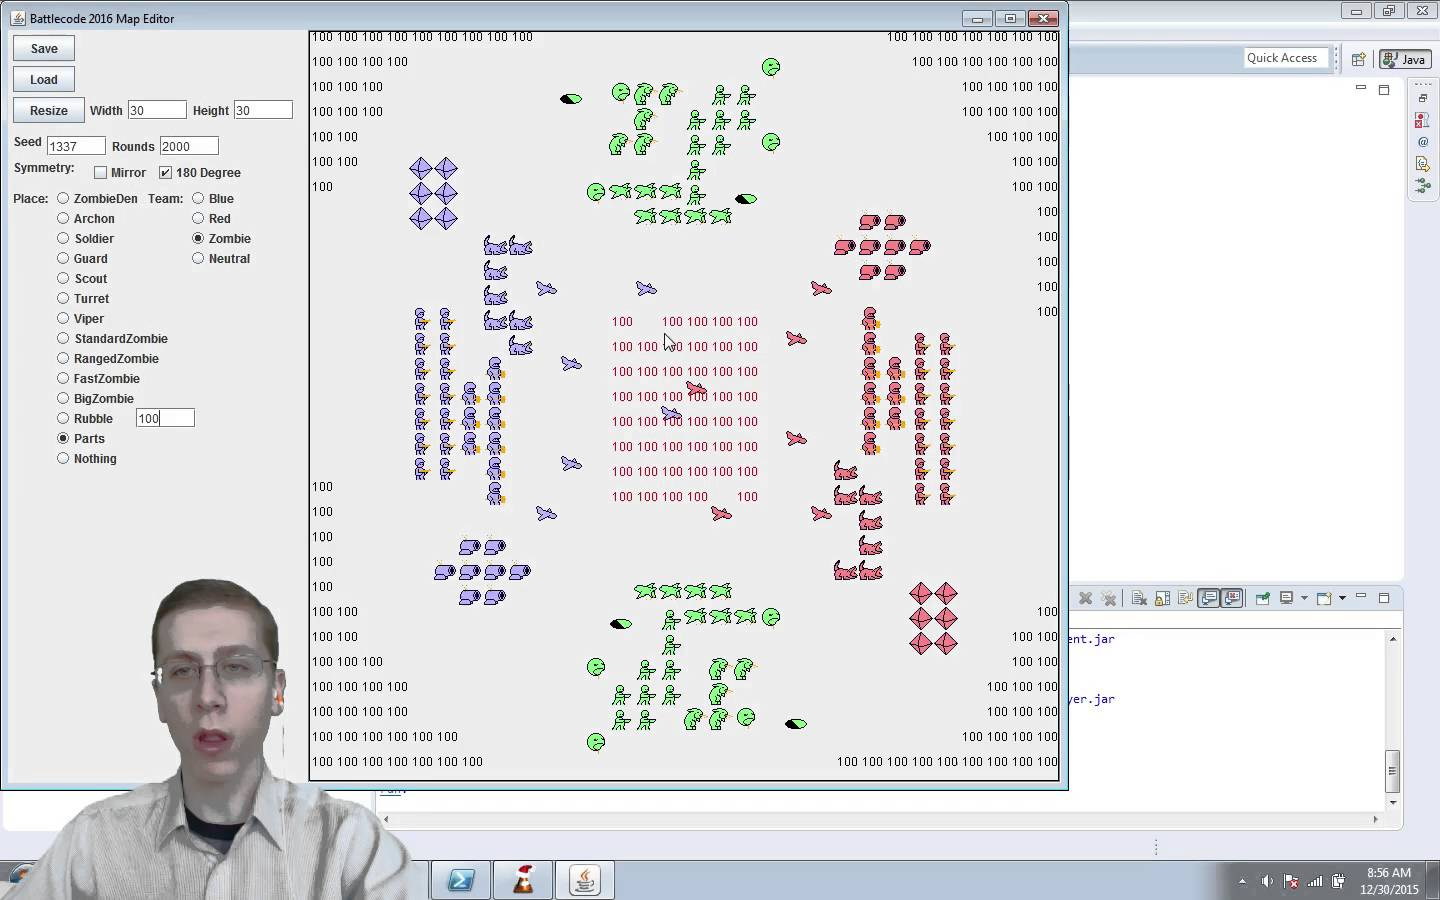
\includegraphics[height =.6\textheight,width=.7\textwidth]{figuras/DAI_motivation01.jpg}
\caption{Ações paralelas, distribuídas, concorrentes ... e tudo coordenado?}
%\label{ag_01}
\end{figure}
    
\end{frame}

%------------------------------------------------------------------------

\begin{frame} %[allowframebreaks=0.9]

  \frametitle{Motivando o \textit{distribuído}}
        
\begin{figure}[!ht]
\centering
%\includegraphics{}
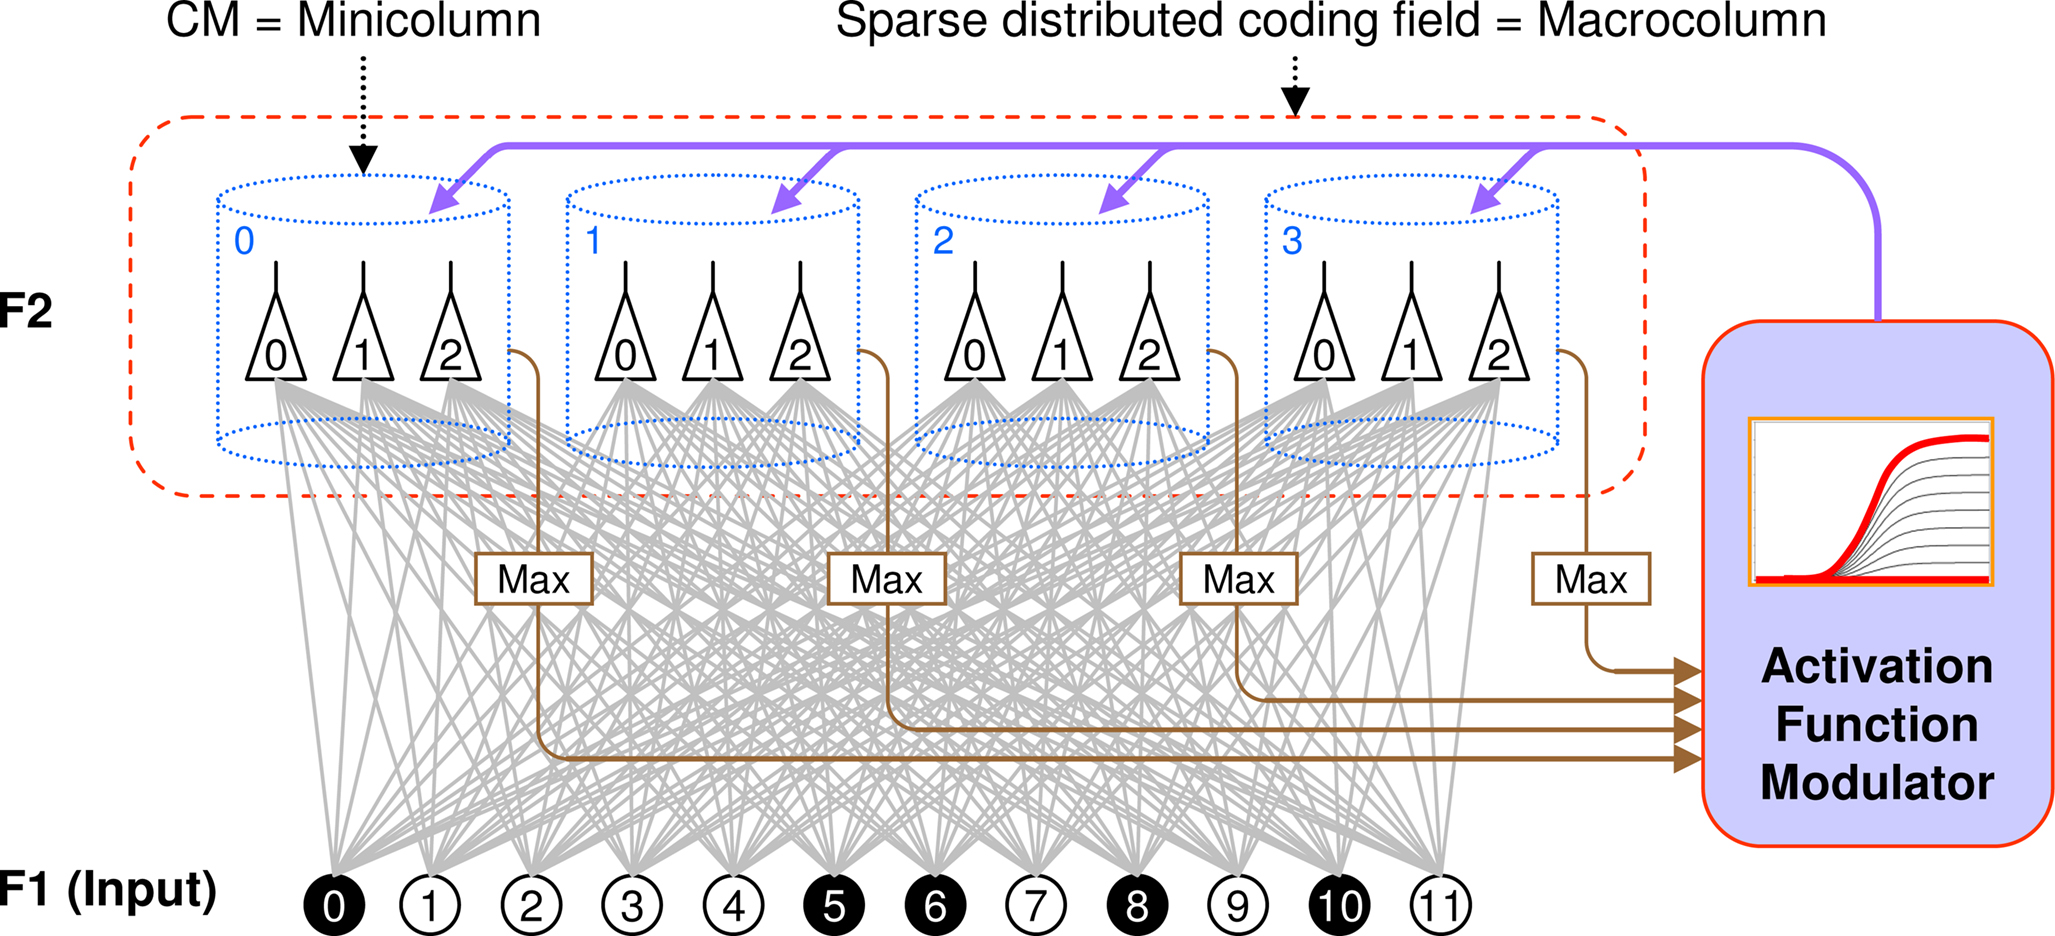
\includegraphics[height =.6\textheight,width=.8\textwidth]{figuras/DAI_motivation02.jpg}
\caption{Mapeando funções via RN -- representações funcionais -- cérebro}
%\label{ag_01}
\end{figure}
    
\end{frame}

%------------------------------------------------------------------------

\begin{frame} %[allowframebreaks=0.9]

  \frametitle{Motivando o \textit{distribuído}}
        
\begin{figure}[!ht]
\centering
%\includegraphics{}
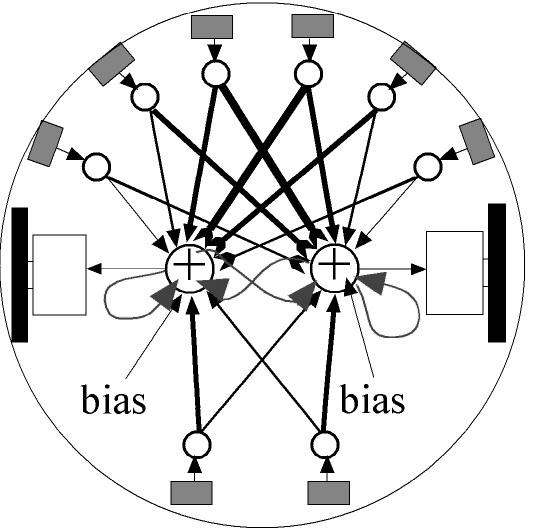
\includegraphics[height =.5\textheight,width=.4\textwidth]{figuras/DAI_motivation03.jpg}
\caption{Robô: mapeando sensores funcionais em atividades motoras $\Rightarrow$ Inspiração 100 \% na entomologia -- ver robôs de Braitenberg}
%\label{ag_01}
\end{figure}
    
\end{frame}




%------------------------------------------------------------------------

\begin{frame} %[allowframebreaks=0.9]

  \frametitle{Arquitetura de  Braitenberg -- 01}
        
\begin{figure}[!ht]
\centering
%\includegraphics{}
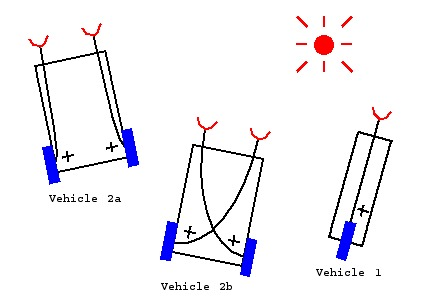
\includegraphics[height =.5\textheight,width=.6\textwidth]{figuras/braitember01.jpg}
\caption{Robôs de Braitenberg}
%\label{ag_01}
\end{figure}
    
\end{frame}
%------------------------------------------------------------------------

\begin{frame} %[allowframebreaks=0.9]

  \frametitle{Arquitetura de  Braitenberg -- 02}
        
\begin{figure}[!ht]
\centering
%\includegraphics{}
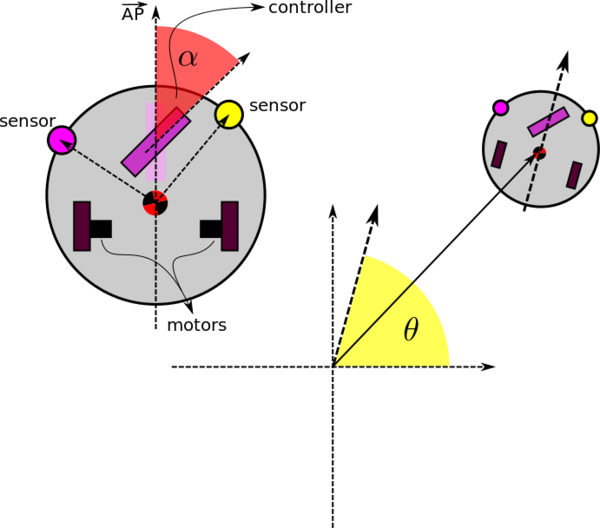
\includegraphics[height =.55\textheight,width=.5\textwidth]{figuras/braitember02.jpg}
\caption{Robôs de Braitenberg}
%\label{ag_01}
\end{figure}
    
\end{frame}
%------------------------------------------------------------------------

\begin{frame} %[allowframebreaks=0.9]

  \frametitle{Arquitetura de  Braitenberg -- 03}
        
\begin{figure}[!ht]
\centering
%\includegraphics{}
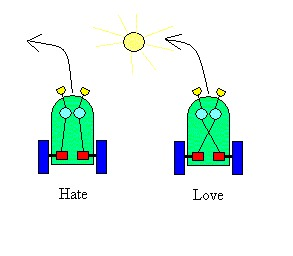
\includegraphics[height =.55\textheight,width=.54\textwidth]{figuras/braitember03.jpg}
\caption{Robôs de Braitenberg -- Inteligência = Comportamento Complexo}
%\label{ag_01}
\end{figure}
    
\end{frame}



%------------------------------------------------------------------------

\begin{frame} %[allowframebreaks=0.9]

  \frametitle{Há muito cálculo \textit{distribuído}, como os processos mentais:}
        
\begin{figure}[!ht]
\centering
%\includegraphics{}
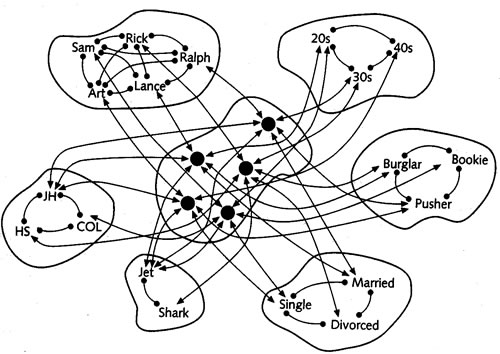
\includegraphics[height =.6\textheight,width=.8\textwidth]{figuras/processamento_mental_01.jpg}
%\caption{Robo: mapeando sensores funcionais em atividades motoras $\Rightarrow$ Inspiração 100 \% na entomologia}
%\label{ag_01}
\end{figure}
    
\end{frame}



%------------------------------------------------------------------------


\begin{frame} %[allowframebreaks=0.9]


\frametitle{Motivando a distribuição:}

\begin{itemize}
  \item Porque o problema é fisicamente distribuído.
  \item Porque o problema é heterogêneo.
  \item Porque o problema só pode ser resolvido pela integração de pontos de vista locais.
  \item Porque precisamos de adaptação a mudanças estruturais...

\end{itemize}

\end{frame}
%------------------------------------------------------------------------


%------------------------------------------------------------------------


\begin{frame} %[allowframebreaks=0.9]

\frametitle{As vantagens da distribuição:}

\begin{itemize}
  \item Maior rapidez na solução dos problemas
  \item Diminuição do \textit{overhead} de comunicação
  \item Maior flexibilidade
  \item Aumento da segurança -- tolerância a falhas
\end{itemize}

\end{frame}
%------------------------------------------------------------------------





\begin{frame}

  \frametitle{Motivando o  \textit{distribuído}}
        
\begin{figure}[!ht]
\centering
%\includegraphics{}
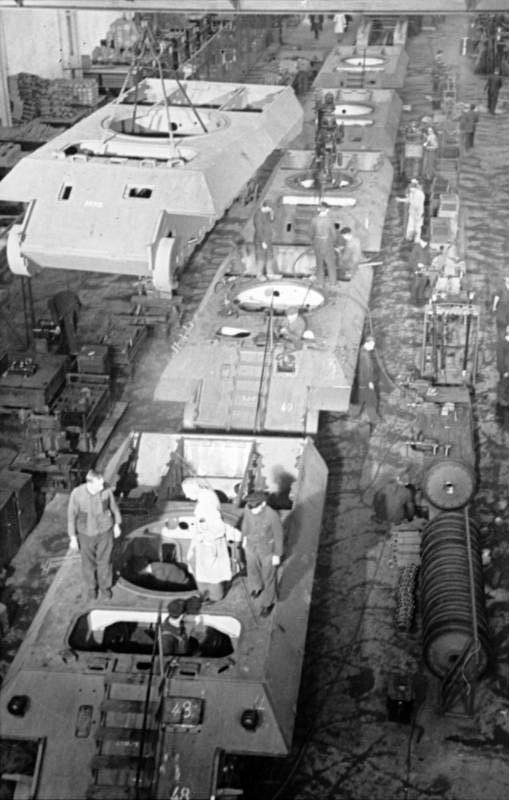
\includegraphics[height =.6\textheight,width=.4\textwidth]{figuras/fabrica_tanques.jpg}
\caption{Ações paralelas, distribuídas, concorrentes ... e tudo planejado!}
%\label{ag_01}
\end{figure}
    
   
\end{frame}





%------------------------------------------------------------------------


\begin{frame} %[allowframebreaks=0.9]


\frametitle{IA Distribuída}

\begin{itemize}
  \item Entidades (ou várias) que interagem sob uma:
  \begin{itemize}
    \item Organização (há uma conexão entre as partes)
     \item Ação 
     \item Interação
  \end{itemize}

     \item Metáfora usada de inteligência: \textcolor{blue}{\textbf{comportamento  social}} (sim, os dos seres animais, incluindo o \textit{homo-sapiens}!)
\end{itemize}


\end{frame}

%------------------------------------------------------------------------

\begin{frame} %[allowframebreaks=0.9]


\frametitle{Resumindo a IAD}

\begin{itemize}
    \item Não é IA paralela (esta é voltada em paralelizar computacionalmente as implementações em IA), nem Sistemas Distribuídos. 
  
    \item Um resolução grupal de problemas, através de  \textit{cooperação} (diferente de \textit{colaboração}).
    
    \item Grande interatividade e capacidade de comunicação.

     \item Organização - meios que garantam a \textit{convergência}: 
      estruturas de autoridade e controle divididos. 

     \item Divisão de conhecimento (nota: \textit{o que é conhecimento?}) e recursos
     
\end{itemize}


\end{frame}

%------------------------------------------------------------------------


\begin{frame} %[allowframebreaks=0.9]


\frametitle{IA Distribuída: 
dois tipos de sistemas}

\begin{itemize}

  \item Resolução Distribuída de Problemas (RDP)
  \begin{itemize}
    \item consciência do objetivo global e divisão clara de tarefas
     \item Exemplos: robótica clássica, busca na Web, gerência de sistemas distribuídos, ...
  \end{itemize}
 
 \item Sistemas Multiagentes (SMA)
    
     \begin{itemize}
       \item não consciência do objetivo global e nem divisão clara de tarefas
       \item Exemplos: n-puzzle, futebol de robôs, balanceamento de carga, robótica, ...

     \end{itemize}

     \end{itemize}
\end{frame}


%------------------------------------------------------------------------


\begin{frame} %[allowframebreaks=0.9]


\frametitle{Porque usar a metáfora de agentes?}

\begin{itemize}
  \item Fornece metodologias de desenvolvimento de sistemas  inteligentes estendendo as de engenharia de software
   \item Fornece visão unificadora das várias sub-áreas da IA 
  \item  Ajuda a embutir a IA em sistemas computacionais 
tradicionais
  \item  Permite tratar melhor a interação com ambiente 
  \item Permite tratamento natural da IA distribuída (distribuir!!!)
  
\end{itemize}


\end{frame}
%------------------------------------------------------------------------


\begin{frame} %[allowframebreaks=0.9]


\frametitle{Ainda RDP $\times$ SMA }

\begin{block}
  
  \begin{description}
    \item[RDP:] 
    \begin{itemize}
      \item Um grupo de especialistas
      \item Habilidades Complementares
      \item Organização Fixa
    \end{itemize}
    
    \item[SMA:]
    
    \begin{itemize}
      \item Agentes podem preexistir
      \item Organização varia em tempo de execução
    \end{itemize}
     
  \end{description}
   
\end{block}

\end{frame}

%------------------------------------------------------------------------


\begin{frame} %[allowframebreaks=0.9]

\frametitle{Fechando esta relação ... RDP $\times$ SMA }

\begin{block}
  
  \begin{description}
    \item[RDP:] 
    \begin{itemize}
      \item RDP é um subconjunto de SMA
      \item Agentes benevolentes, concebidos em conjunto
    \end{itemize}
    
    \item[SMA:]
    \begin{itemize}
      \item SMA é base para RDP
      \item Implementação descentralizada de várias propriedades
    \end{itemize}
     
  \end{description}
   
\end{block}

\end{frame}

%------------------------------------------------------------------------

%------------------------------------------------------------------------


\begin{frame} %[allowframebreaks=0.9]

\frametitle{Um Sistema Multiagente (SMA) formal}

\begin{block}{Um SMA é um sistema que possui os seguintes elementos:}
  \begin{itemize}
    \item Um ambiente: $E$
    \item Um conjunto de objetos: $O$
    \item Um conjunto de Agentes: $A$ ($A\subseteq O$)
    \item Um conjunto de relações $R$, a qual estabelece
    conexões entre os objetos
    \item Um conjunto de operações: $O_p$
    \item Operadores que representam os resultados das operações em $O_p$
     e as reações do ambiente a eles.
       
  \end{itemize}
   
\end{block}

\textcolor{red}{Construa uma tupla para esta formalização}


\end{frame}



\begin{frame} %[allowframebreaks=0.9]

\frametitle{Isto é:}

\begin{block}{Um SMA:}
  \begin{itemize}

   \item Consiste de uma coleção de componentes autônomos, com objetivos particulares
    \item Que se interrelacionam

\begin{itemize}
  \item De acordo com uma Organização
  \item Interagindo, negociando  e coordenando esforços para resolver tarefas 
  \end{itemize}  
  \end{itemize}
   
\end{block}

\end{frame}

%------------------------------------------------------------------------

\begin{frame} %[allowframebreaks=0.9]

  \frametitle{Exemplos de uso de SMAs:}
        
\begin{figure}[!ht]
\centering
%\includegraphics{}
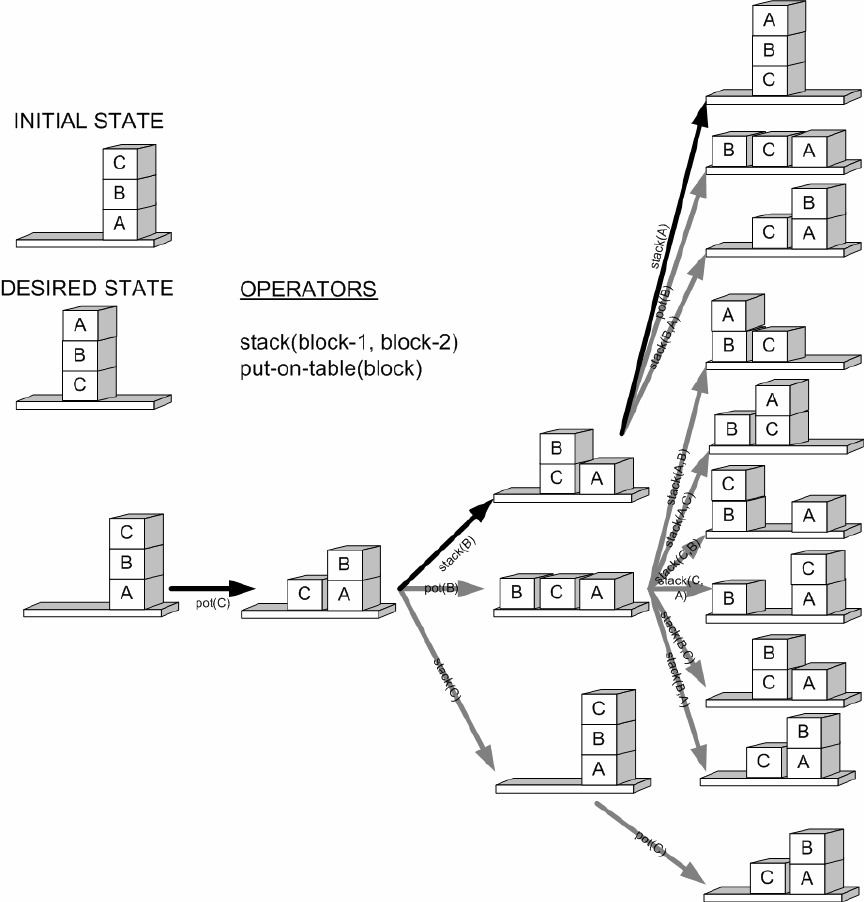
\includegraphics[height =.6\textheight,width=.7\textwidth]{figuras/original_example_SMAs01.jpg}
\caption{\textit{Mundo dos blocos} -- um agente neste caso é previsível}
%\label{ag_01}
\end{figure}
    
\end{frame}

%------------------------------------------------------------------------

\begin{frame} %[allowframebreaks=0.9]

  \frametitle{Exemplos de uso de SMAs:}
        
\begin{figure}[!ht]
\centering
%\includegraphics{}

\includegraphics[height =.5\textheight,width=.7\textwidth]{figuras/example_SMAs01.jpg}
\caption{\textit{Mundo dos blocos} com vários robôs}
%\label{ag_01}
\end{figure}
    
\end{frame}

%%---------------------------------------------------------------------
\begin{frame} %[allowframebreaks=0.9]

  \frametitle{Exemplos de uso de SMAs:}
        
\begin{figure}[!ht]
\centering
%\includegraphics{}
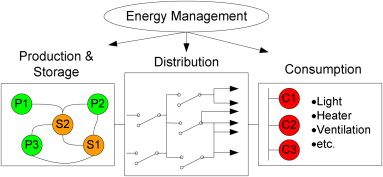
\includegraphics[height =.6\textheight,width=.7\textwidth]{figuras/example_SMAs02.jpg}
\caption{As chaves comutadoras são agentes?}
%\label{ag_01}
\end{figure}
    
\end{frame}
%%---------------------------------------------------------------------

\begin{frame} %[allowframebreaks=0.9]

  \frametitle{Exemplos de uso de SMAs:}
        
\begin{figure}[!ht]
\centering
%\includegraphics{}
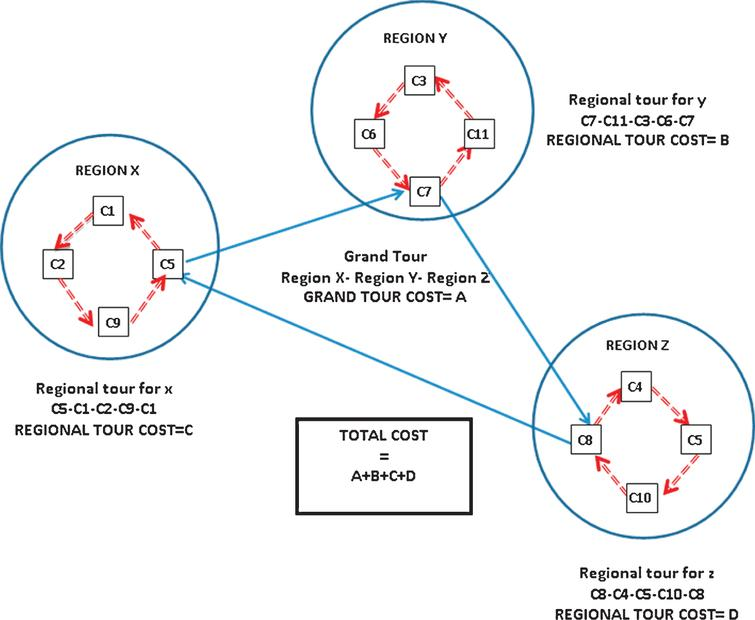
\includegraphics[height =.6\textheight,width=.7\textwidth]{figuras/example_SMAs03.jpg}
\caption{Removendo a dinâmica das regiões este é um exemplo de RDP}
%\label{ag_01}
\end{figure}
    
\end{frame}
%%---------------------------------------------------------------------


%%---------------------------------------------------------------------
\begin{frame} %[allowframebreaks=0.9]

\frametitle{Em resumo... é uma boa idéia quando...:}


\begin{itemize}
  \item Precisamos manter a autonomia das sub-partes
  \item As interações são complexas
  \item Não é possível descrever o problema \textit{a priori}.
\end{itemize}
\end{frame}

\begin{frame} %[allowframebreaks=0.9]

\frametitle{E as  vantagens...:}

\begin{block}{}
\begin{enumerate}
  \item Maior rapidez na solução dos problemas
  \item Diminuição do \textit{overhead} de comunicação
  \item Maior flexibilidade
  \item Aumento da segurança -- tolerância a falhas
\end{enumerate}

\begin{itemize}
  \item \textcolor{blue}{Uma vez definidos e motivados, agora faltam os detalhes 
de como implementar tudo isto!}

 \item \textcolor{blue}{Ver seção de projetos de SMAs!}

\end{itemize}
\end{block}

\end{frame}


%------------------------------------------------------------------------

\begin{frame} %[allowframebreaks=0.9]

  \frametitle{Epílogo: um agente já tem uma realidade \textit{complexa}:}
        
\begin{figure}[!ht]
\centering
%\includegraphics{}
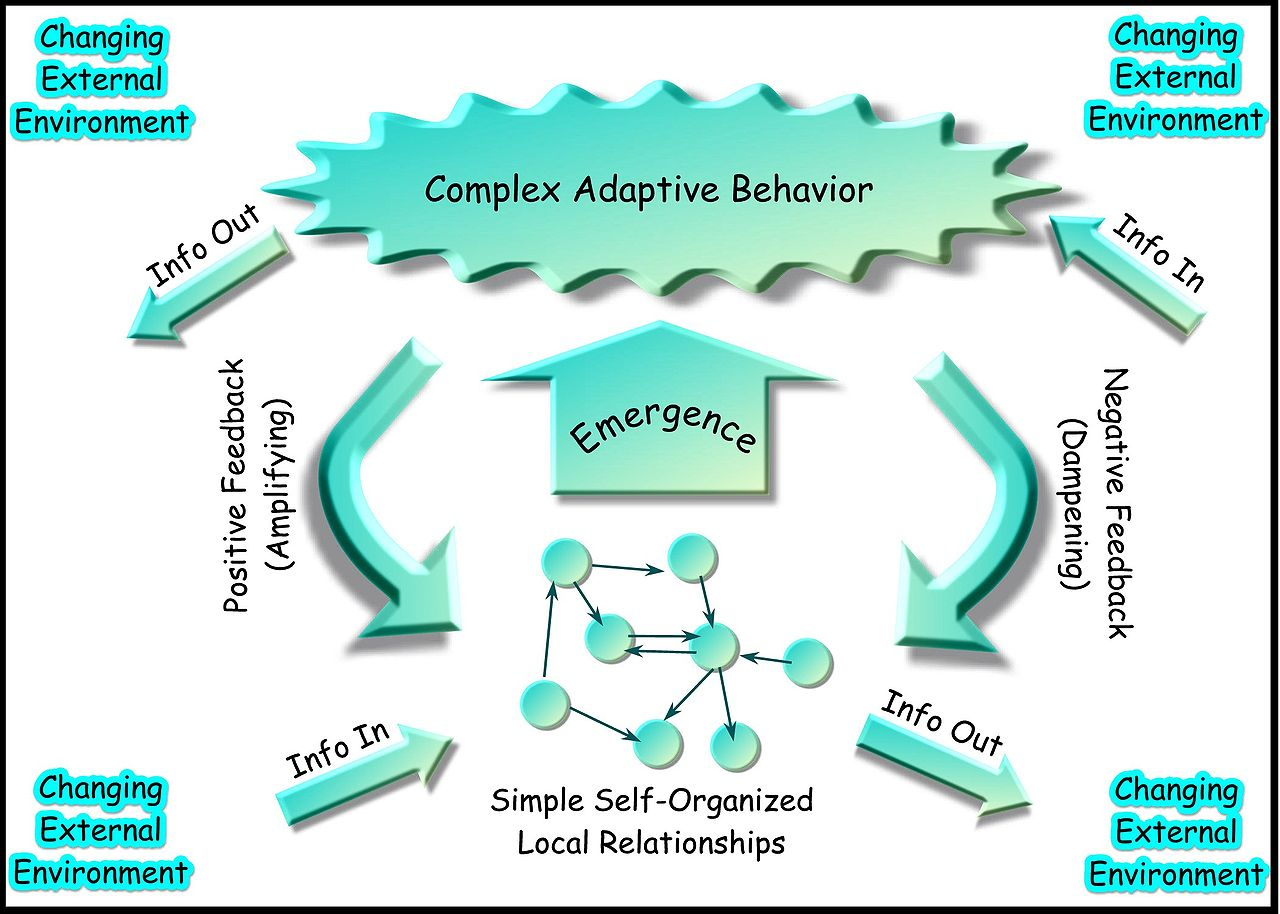
\includegraphics[height =.6\textheight,width=.7\textwidth]{figuras/complex-adaptive-system.jpg}
\caption{Um agente e sua \textit{sociedade de agentes} ...}
%\label{ag_01}
\end{figure}
    
\end{frame}








\begin{frame} %[allowframebreaks=0.9]

 \frametitle{Resumo do capítulo}

\begin{enumerate}
  \item Vocabulário
 \item Diferença de SMAs com RDPs  na IAD
  \item Soluções de SMAs são atrativas porquê
    
    \item Falta: Coordenação etc
        \item Falta: Planejamento etc
     \item Falta: projetar  SMAs     
  
\end{enumerate}


\end{frame}
